\documentclass[12pt]{article}
\usepackage[margin=1in]{geometry}                % See geometry.pdf to learn the layout options. There are lots.
\geometry{letterpaper}                   % ... or a4paper or a5paper or ... 
%\geometry{landscape}                % Activate for for rotated page geometry
\usepackage[parfill]{parskip}    % Activate to begin paragraphs with an empty line rather than an indent

%%%%%%%%%%%%%%%%%%%%
\newcommand{\hide}[1]{}

\usepackage{natbib}
\usepackage{xcolor}
\usepackage{url}
\usepackage{hyperref}
\usepackage{mathtools}

\hide{
\usepackage{amscd}
\usepackage{amsfonts}
\usepackage{amsmath}
\usepackage{amssymb}
\usepackage{amsthm}
\usepackage{cases}		 
\usepackage{cutwin}
\usepackage{enumerate}
\usepackage{enumitem}
\usepackage{epstopdf}
\usepackage{graphicx}
\usepackage{ifthen}
\usepackage{lipsum}
\usepackage{mathrsfs}	
\usepackage{multimedia}
\usepackage{wrapfig}
}
\bibliographystyle{humanbio}

	 
%\input{/usr/local/LATEX/Lee_newcommands.tex}
\newcommand{\itemlist}[1]{\begin{itemize}#1\end{itemize}}
\newcommand{\enumlist}[1]{\begin{enumerate}#1\end{enumerate}}
\newcommand{\desclist}[1]{\begin{description}#1\end{description}}

\newcommand{\Answer}[1]{\begin{quote}{\color{blue}#1}\end{quote}}
\newcommand{\AND}{\wedge}
\newcommand{\OR}{\vee}
\newcommand{\ra}{\rightarrow}
\newcommand{\lra}{\leftrightarrow}

\title {{\bf Project 1: Distributed Coordination Function} \\
\large{ECE 578: Fundamentals of Computer Networks}}

\author{Lena Voytek and Mitchell Dzurick}
\date{10/22/2019}


\begin{document}
\maketitle{}

\section*{Introduction:}

    This project models four different scenarios where multiple nodes are transmitting packets over an 802.11 network protocol. The first two are based on a network where four nodes are in a single collision domain with two of the nodes transmitting frames in a Poisson-distributed manner. One of them uses generic CSMA/CA while the other also implements virtual carrier sensing. The second set are based on a network where the two nodes are sending to the same receiver while being hidden to one another. Once again, on uses CSMA/CA, while the other implements virtual carrier sensing.
    \par
    The workload was split evenly between the two group members. Most of it was completed as a combined effort between them at the same time, such as the determined code structure and documentation. Lena was responsible of the logic of each simulation and the creation of a general Poisson arrival function. Mitchell was in charge of developing an automated graph creation system and creating a system to build and execute all simulations while outputting to the proper files.
    \par
    Development for the project consisted of the languages C, Make, CMake, Gnuplot, shell scripting, and \LaTeX{}. The actual simulation code was created in C using a set of six files and structs for nodes. Make and CMake were used to automatically compile and run simulations while using the CLion IDE. Gnuplot scripts were developped to automatically create each graph and export them to PNG files. Shell scripting was used to easily run the graph creation scripts. Finally, \LaTeX{} was used to create this document. For more specifics and the actual code, see the project on Github at \\
    \textcolor{blue}{ \href{https://github.com/lvoytek/ECE578/tree/master/DistributedCoordinationFunction}{https://github.com/lvoytek/ECE578/tree/master/DistributedCoordinationFunction}}.

\clearpage

\section{Throughput T}

    \renewcommand{\labelenumi}{{\bf\alph{enumi})}}
    \begin{enumerate}
        \item { 
            {\bf Node A:} Throughput T (Kbps) vs. rate \(\lambda{}\) (frames/sec) for scenarios A and B, and CSMA implementations 1 and 2.
            
            \begin{figure}[!htb]
                \centering
                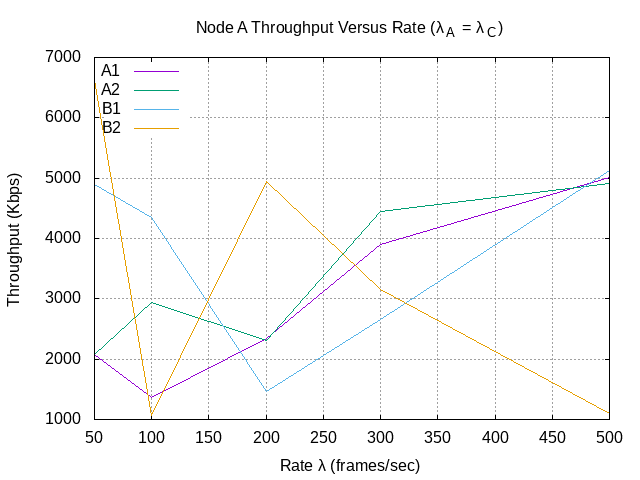
\includegraphics[width=5in]{1A.png}
                \caption{Node A Throughput when \(\lambda{} = \lambda{}_A = \lambda{}_C\) }
                \label{fig:1A}
            \end{figure}
            
            In general, for each Node A using a control \(\lambda{}\) value equal to that of C, the throughput begins with a decrease, followed by a gradual increase as the frame rate increases.
        }
        
\clearpage

        \item {
            {\bf Node C:} Throughput T (Kbps) vs. rate \(\lambda{}\) (frames/sec) for scenarios A and B, and CSMA implementations 1 and 2.
            
            \begin{figure}[!htb]
                \centering
                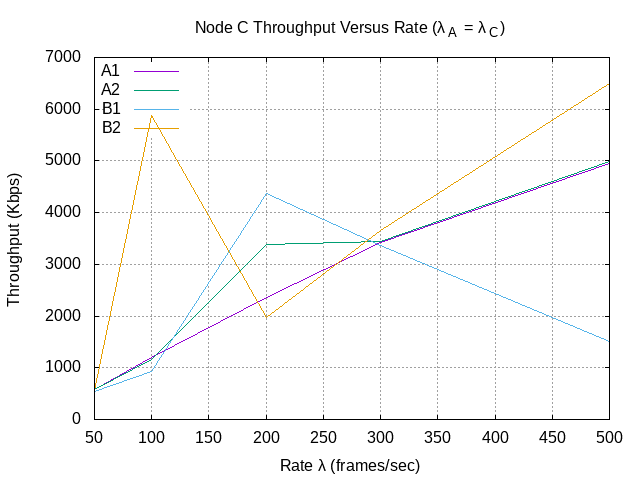
\includegraphics[width=5in]{1B.png}
                \caption{Node C Throughput when \(\lambda{} = \lambda{}_A = \lambda{}_C\) }
                \label{fig:1B}
            \end{figure}

            ----Explain 1b----
        }
        
\clearpage
        \item {
            {\bf Node A:} Throughput T (Kbps) vs. rate \(\lambda{}\) (frames/sec) for scenarios A and B, and CSMA implementations 1 and 2, when \(\lambda{}_A = 2\lambda{}\).
            
            \begin{figure}[!htb]
                \centering
                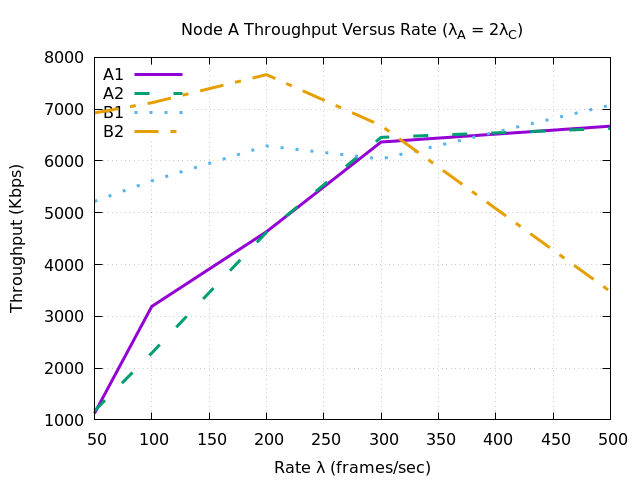
\includegraphics[width=5in]{1C.png}
                \caption{Node A Throughput when \(\lambda{}_A = 2\lambda{}, \lambda{}_C = \lambda{}\) }
                \label{fig:1C}
            \end{figure}

            ----Explain 1c----
        }
        
\clearpage
        \item {
            {\bf Node C:} Throughput T (Kbps) vs. rate \(\lambda{}\) (frames/sec) for scenarios A and B, and CSMA implementations 1 and 2, when \(\lambda{}_A = 2\lambda{}\).
            
            \begin{figure}[!htb]
                \centering
                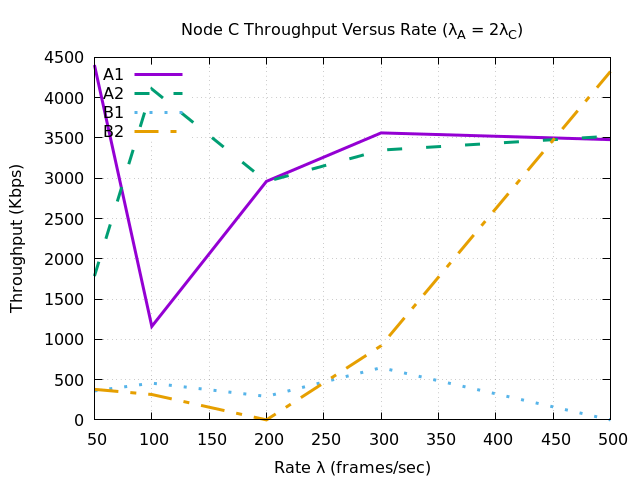
\includegraphics[width=5in]{1D.png}
                \caption{Node C Throughput when \(\lambda{}_A = 2\lambda{}, \lambda{}_C = \lambda{}\) }
                \label{fig:1D}
            \end{figure}

            ----Explain 1d----
        }
        
    \end{enumerate}
        
\clearpage        
\section{Collisions N}

    \begin{enumerate}
    
        \item {
            {\bf Node A:} Number of collisions N vs. rate \(\lambda{}\) (frames/sec) for scenarios A and B, and CSMA implementations 1 and 2.
            
            \begin{figure}[!htb]
                \centering
                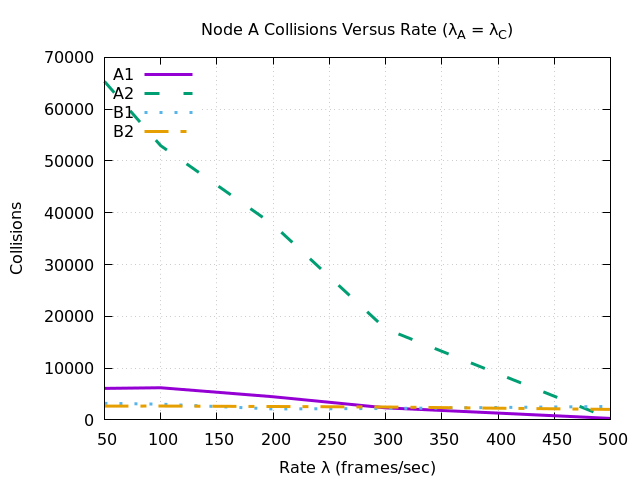
\includegraphics[width=5in]{2A.png}
                \caption{Node A Collisions when \(\lambda{} = \lambda{}_A = \lambda{}_C\) }
                \label{fig:2A}
            \end{figure}

            ----Explain 2A----
        }    
    
    
\clearpage  
        \item {
            {\bf Node C:} Number of collisions N vs. rate \(\lambda{}\) (frames/sec) for scenarios A and B, and CSMA implementations 1 and 2.
            
            \begin{figure}[!htb]
                \centering
                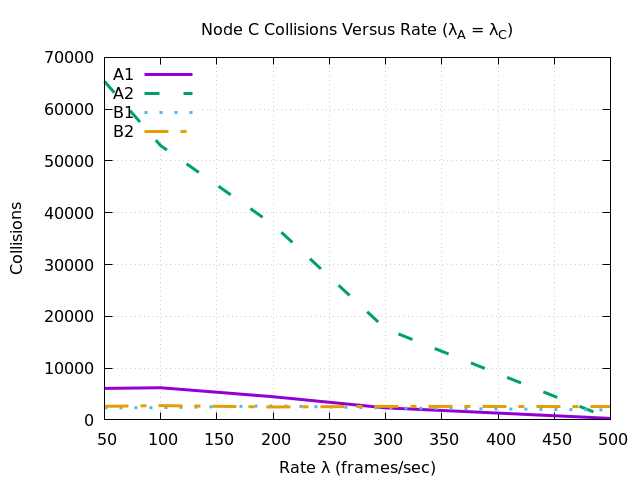
\includegraphics[width=5in]{2B.png}
                \caption{Node C Collisions when \(\lambda{} = \lambda{}_A = \lambda{}_C\) }
                \label{fig:2B}
            \end{figure}

            ----Explain 2B----
        }    
\clearpage  
        \item {
            {\bf Node A:} Number of collisions N vs. rate \(\lambda{}\) (frames/sec) for scenarios A and B, and CSMA implementations 1 and 2, when \(\lambda{}_A = 2\lambda{}\).
            
            \begin{figure}[!htb]
                \centering
                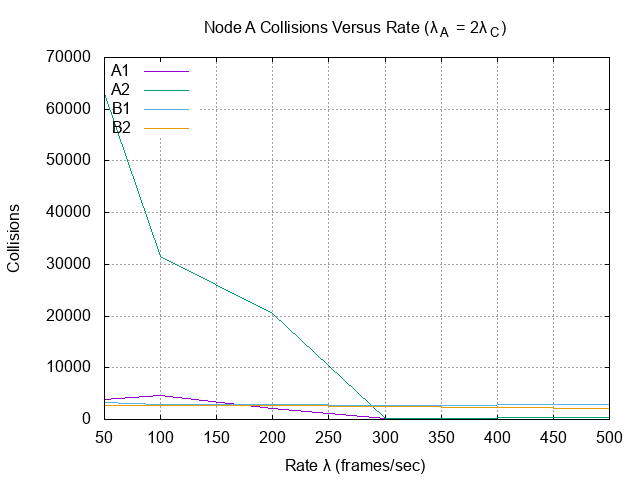
\includegraphics[width=5in]{2C.png}
                \caption{Node A Collisions when \(\lambda{}_A = 2\lambda{}, \lambda{}_C = \lambda{}\) }
                \label{fig:2C}
            \end{figure}

            ----Explain 2C----
        }        
    
\clearpage  
        \item {
            {\bf Node C:} Number of collisions N vs. rate \(\lambda{}\) (frames/sec) for scenarios A and B, and CSMA implementations 1 and 2, when \(\lambda{}_A = 2\lambda{}\).
            
            \begin{figure}[!htb]
                \centering
                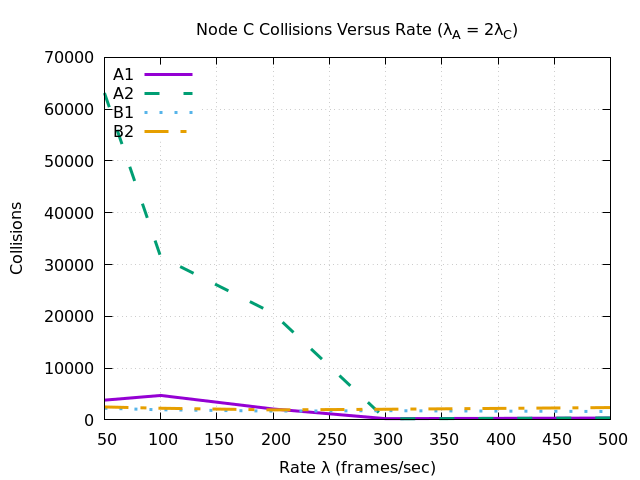
\includegraphics[width=5in]{2D.png}
                \caption{Node C Collisions when \(\lambda{}_A = 2\lambda{}, \lambda{}_C = \lambda{}\) }
                \label{fig:2D}
            \end{figure}

            ----Explain 2D----
        }        
    
    
    \end{enumerate}
    
    
\clearpage
    \section{Fairness Index FI}

    \begin{enumerate}
    
        \item {
            Fairness Index FI vs. rate \(\lambda{}\) (frames/sec) for scenarios A and B, and CSMA implementations 1 and 2.
            
            \begin{figure}[!htb]
                \centering
                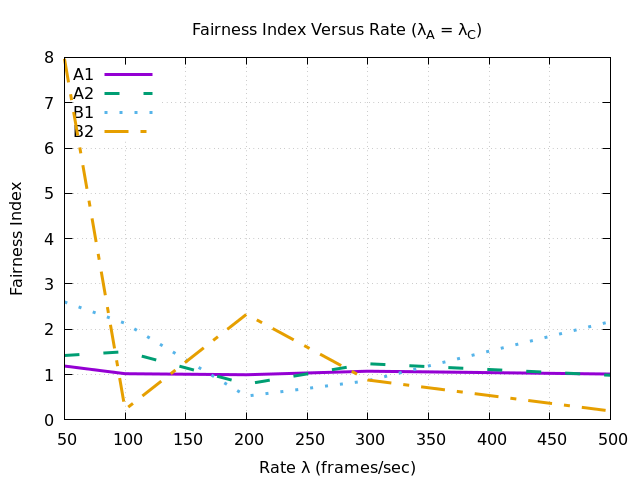
\includegraphics[width=5in]{3A.png}
                \caption{Fairness Index when \(\lambda{} = \lambda{}_A = \lambda{}_C\) }
                \label{fig:3A}
            \end{figure}

            ----Explain 3A----
        }    
    
    
\clearpage  
        \item {
            Fairness Index FI vs. rate \(\lambda{}\) (frames/sec) for scenarios A and B, and CSMA implementations 1 and 2, when \(\lambda{}_A = 2\lambda{}\).
            
            \begin{figure}[!htb]
                \centering
                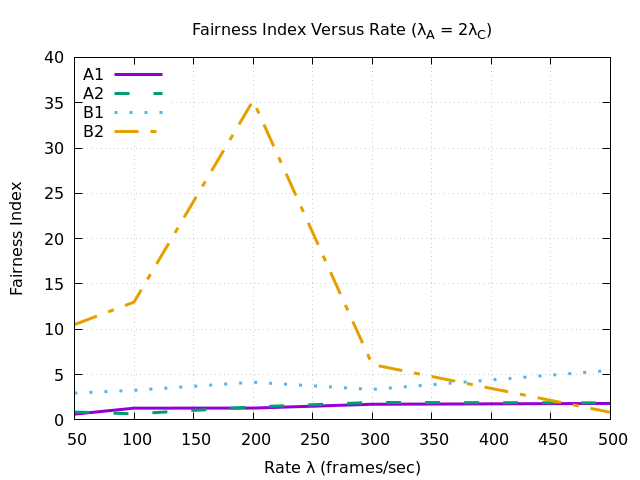
\includegraphics[width=5in]{3B.png}
                \caption{Fairness Index when \(\lambda{}_A = 2\lambda{}, \lambda{}_C = \lambda{}\) }
                \label{fig:3B}
            \end{figure}

            ----Explain 3B----
        }    
    \end{enumerate}
\end{document}  
%%%%%%%%%%%%%%%%%%%%%%%%%%%%%%%%%%%%%%%%%%%%%%